\documentclass{article}
\usepackage[utf8]{inputenc}
\usepackage{pgfplots}
\pgfplotsset{width=10cm,compat=1.9}
\usepackage{amsmath,amssymb,amsthm}
\usepackage{gensymb}
\usepackage{graphicx}
\usepackage{float}
\usepackage{xcolor}
\usepackage{blindtext}
\usepackage{hyperref}
\usepackage[margin=1in]{geometry}
\hypersetup{
    colorlinks=true,
    linkcolor=blue,
    filecolor=magenta,      
    urlcolor=cyan,
    pdftitle={Overleaf Example},
    pdfpagemode=FullScreen,
    }
\usepackage[slovene]{babel}

\newcounter{example}[section]
\newenvironment{example}[1][]{\refstepcounter{example}\par\medskip
   \noindent \textbf{Naloga~\theexample. #1} \rmfamily}{\medskip}

\newtheorem*{zgled}{Zgled}

\title{Trigonometrija}
\author{Bor Bregant}
\date{\vspace{-5ex}}

\begin{document}

\maketitle

\[\text{V pravokotnem trikotniku velja:}\]
\[\sin\phi=\frac{\text{nepriležna}}{\text{hipotenuza}}\qquad \cos\phi=\frac{\text{priležna}}{\text{hipotenuza}}\qquad \tan\phi=\frac{\text{nepriležna}}{\text{priležna}}\qquad \cot\phi=\frac{\text{priležna}}{\text{nepriležna}}\]

\[\tan\phi=\frac{\sin\phi}{\cos\phi}\qquad \cot\phi=\frac{\cos\phi}{\sin\phi}\]

\[\cos(\frac{\pi}{2}-\phi)=\sin\phi \qquad \sin(\frac{\pi}{2}-\phi)=\cos\phi\qquad \tan(\frac{\pi}{2}-\phi)=\cot\phi\qquad \cot(\frac{\pi}{2}-\phi)=\tan\phi\]

\[\sin^2x+\cos^2x=1\qquad 1+\tan^2x=\frac{1}{\cos^2x}\qquad 1+\cot^2x=\frac{1}{\sin^2x}\]

\section{Enotska krožnica}

1 radian je kot, ki pripada loku, dolgemu natanko polmer krožnice.

\begin{figure}[H]

\includegraphics[width=0.4\textwidth]{trigonometrija.radiani.pdf}
\centering
\end{figure}

\begin{figure}[H]
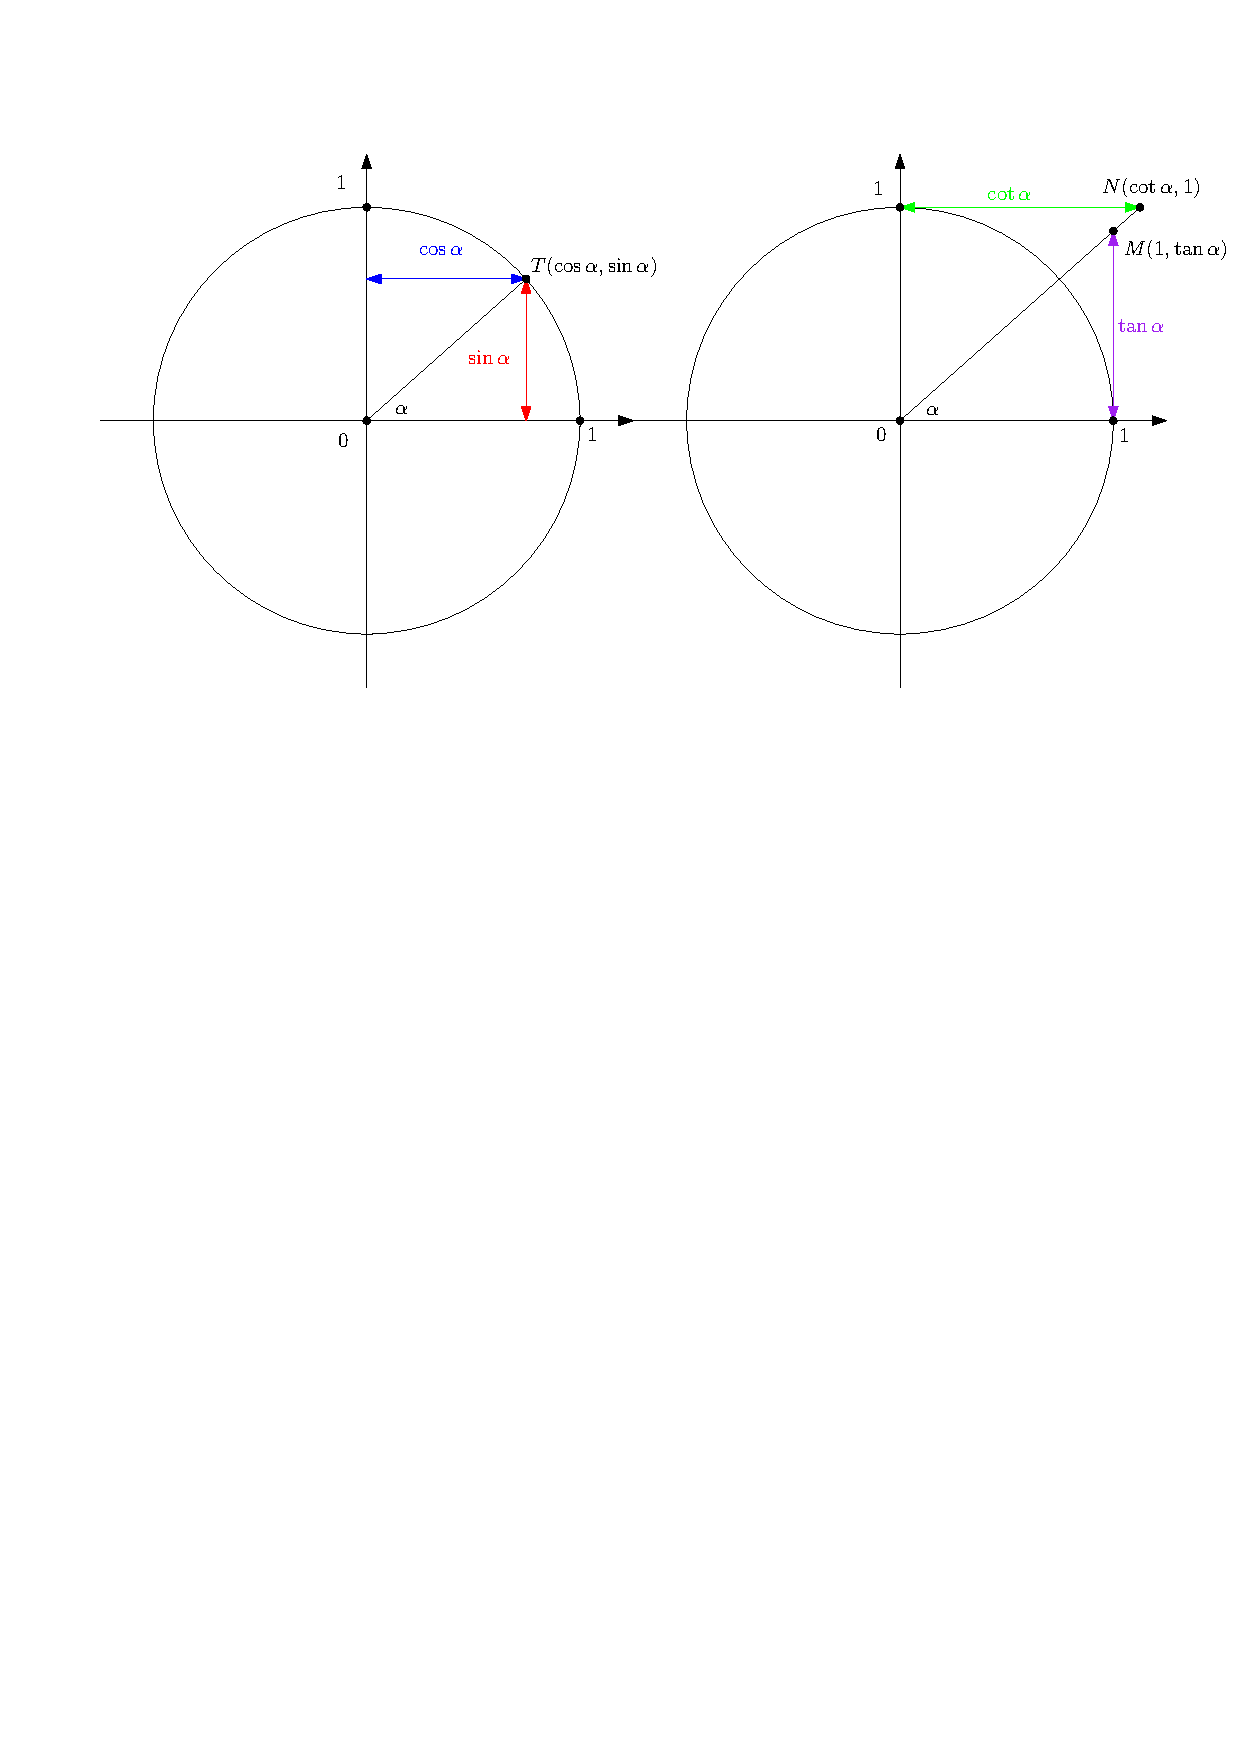
\includegraphics[width=0.8\textwidth]{trigonometrija.enotska.pdf}
\centering
\end{figure}

\begin{tabular*}{\linewidth}[b]{*{6}{|c @{\extracolsep\fill}}|}
\hline  Kot $\angle^\circ \rightarrow$   &0$^\circ$& 30$^\circ$ & 45$^\circ$ & 60$^\circ$ & 90$^\circ$
\\ $\downarrow$ Funkcija $\angle ^\circ$ &  &  &  &  & \\ 
\hline $\sin \theta$ & 0 & $\dfrac{1}{2}$ &$\dfrac{1}{\sqrt{2}}$ & $\dfrac{\sqrt{3}}{2}$& 1\\[15pt]
\hline $\cos \theta$ & 1 & $\dfrac{\sqrt{3}}{2}$ &$\dfrac{1}{\sqrt{2}}$ & $\dfrac{1}{2}$& 0\\ 
\hline $\tan \theta$ & 0 & $\dfrac{{1}}{\sqrt{3}}$ &1  & $\sqrt{3}$ & ND\\
\hline
$\cot \theta$ & ND & $\sqrt{3}$ &1 & $\dfrac{{1}}{\sqrt{3}}$ & 0 \\ \hline
\end{tabular*}


Iz enotske krožnice preberemo še naslednje zveze:

\[\sin(\pi-\phi)=\sin\phi\qquad \cos(\pi-\phi)=-\cos\phi \qquad \tan(\pi-\phi)=-\tan\phi\qquad \cot(\pi-\phi)=-\cot\phi\]

\[\sin(\pi+\phi)=-\sin\phi\qquad \cos(\pi+\phi)=-\cos\phi \qquad \tan(\pi+\phi)=\tan\phi\qquad \cot(\pi+\phi)=\cot\phi\]
\[\sin(-x)=-\sin(x) \qquad \cos(-x)=\cos x \qquad \tan(-x)=-\tan(x) \qquad \cot(-x)=-\cot x\]

Periodičnost ($k\in \mathbb{Z}$):

\[\sin(x+2k\pi)=\sin x \qquad \cos(x+2k\pi)=\cos x\]
\[\tan(x+k\pi)=\tan x \qquad \cot(x+k\pi)=\cot x\]

\begin{zgled}
    Natančno izračunajmo $\sin\frac{10\pi}{3},\ \tan(-\frac{5\pi}{4}),\ \cos(-\frac{5\pi}{6})$.
\end{zgled}
\begin{zgled}
    Natančno izračunajmo $\cos\alpha$, če je $\alpha$ v tretjem kvadrantu in $\sin\alpha=-\frac{1}{4}$
\end{zgled}

\begin{example}
    \textcolor{red}{331ab}, \fbox{339a}bcd, \fbox{343}-347, \fbox{355a}b, 361ac, \fbox{372a}bc,
\end{example}

\section{Grafi kotnih funkcij}

\begin{figure}[H]
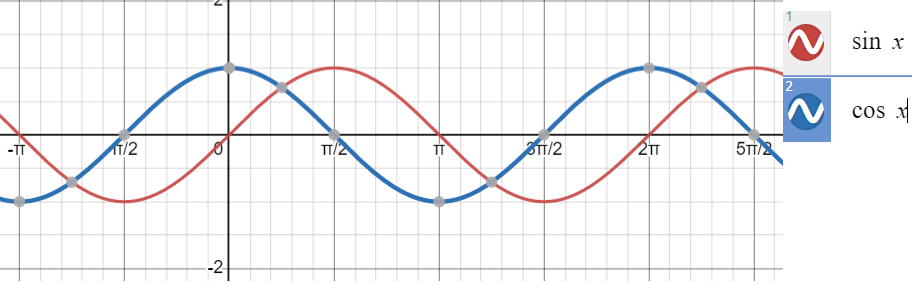
\includegraphics[width=1\textwidth]{trigonometrija.grafsincos.png}
\centering
\end{figure}

\begin{table}[H]
\begin{tabular}{l|l|l}
\begin{tabular}[c]{@{}l@{}}Funkcija $\rightarrow$\textbackslash{}\textbackslash{}\\ $\downarrow$ Lastnosti\end{tabular} & $\sin x$                              & $\cos x$                                                                     \\ \hline
$D_f$                                                                                                                   & $\mathbb{R}$                          & $\mathbb{R}$                                                                 \\
$Z_f$                                                                                                                   & $[-1,1]$                              & $[-1,1]$                                                                     \\
Ničle                                                                                                                   & $x=k\pi$                              & $x=\frac{\pi}{2}+k\pi$                                                       \\
Začetna vrednost                                                                                                        & $f(0)=0$                              & $f(0)=1$                                                                     \\
Max                                                                                                                     & $x_{\text{max}}=\frac{\pi}{2}+2k\pi$  & $x_{\text{max}}=2k\pi$                                                       \\
Min                                                                                                                     & $x_{\text{min}}=\frac{3\pi}{2}+2k\pi$ & $x_{\text{min}}=\pi+2k\pi$ \\
Sodost/lihost                                                                                                           & Liha                                  & Soda                                                                         \\
Ime                                                                                                                     & Sinusoida                             & Sinusoida                                                                    \\
Perioda                                                                                                                 & $2\pi$                                & $2\pi$                                                                       \\
Naraščanje/padanje                                                                                                      & Zapiši sam                            & Zapiši sam                                                                  
\end{tabular}
\caption{$k\in \mathbb{R}$}
\end{table}

\begin{zgled}
    Izračunajmo ničle in maksimume funkcije $f(x)=-\cos x+\frac{1}{2}$ na $[-2\pi,3\pi]$.
\end{zgled}

\begin{figure}[H]
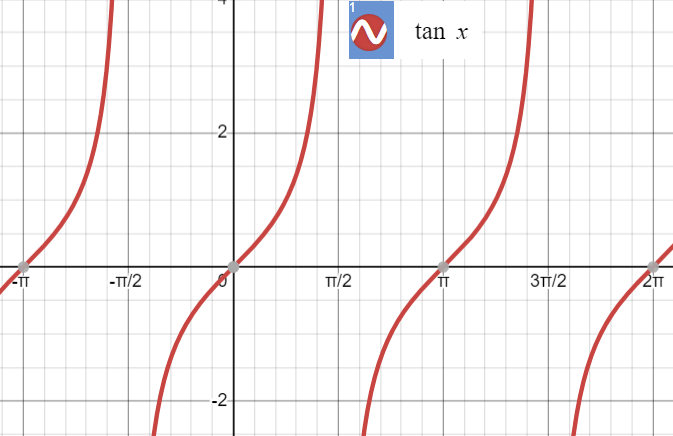
\includegraphics[width=0.6\textwidth]{trigonometrija.graftan.png}
\centering
\end{figure}


\begin{table}[H]
\begin{tabular}{l|l|l}
\begin{tabular}[c]{@{}l@{}}Funkcija $\rightarrow$\textbackslash{}\textbackslash{}\\ $\downarrow$ Lastnosti\end{tabular} & $\tan x$                                     & $\cot x$                       \\ \hline
$D_f$                                                                                                                   & $\mathbb{R}\backslash\{\frac{\pi}{2}+k\pi\}$ & $\mathbb{R}\backslash\{k\pi\}$ \\
$Z_f$                                                                                                                   & $\mathbb{R}$                                 & $\mathbb{R}$                   \\
Ničle                                                                                                                   & $x=k\pi$                                     & $x=\frac{\pi}{2}+k\pi$         \\
Poli (navpične asimpt.)                                                                                                 & $x=\frac{\pi}{2}+k\pi$                       & $x=k\pi$                       \\
Začetna vrednost                                                                                                        & $f(0)=0$                                     & Ni definirana                  \\
Sodost/lihost                                                                                                           & Liha                                         & Liha                           \\
Perioda                                                                                                                 & $\pi$                                        & $\pi$                          \\
Naraščanje/padanje                                                                                                      & Odsekoma naraščajoča                         & Odsekoma padajoča              \\
Omejenost                                                                                                               & Neomejena                                    & Neomejena                     
\end{tabular}
\caption{$k\in\mathbb{R}$}
\end{table}

\begin{zgled}
    Izračunajmo ničle in osnovno periodo $f(x)=2\tan 3x$.
\end{zgled}

\subsection{Transformacije kotnih funkcij}

\[y=A\sin(B(x-C))+D\]

\begin{table}[H]
\begin{tabular}{l|l|l|l}
Parameter                & Ime       & Transformacija                                                                                                                          & Opomba                                                 \\ \hline
$A$                      & Amplituda & Razteg $\updownarrow$                                                                                                                   & $A>1$ razteg, $0<A<1$ skrčitev, $A<0$ še zrcaljenje    \\
$B$                      & Frekvenca & Razteg $\leftrightarrow$                                                                                                                & $B>1$ zgostitev, $0<B<1$ redčitev, $B<0$ še zrcaljenje \\
$C$                      &           & Premik $\leftrightarrow$                                                                                                                & Pazi na $-$. Če $C>0$ se premakne desno       \\
$D$                      &           & Premik $\updownarrow$                                                                                                                   &                                                        \\ \hline
Premik za vektor&           &                                                                                                                                         &                                                        \\
Absolutna vrednost       &           & \begin{tabular}[c]{@{}l@{}}Kar je spodaj zrcalimo gor ali\\ Del grafa $x>0$ zrcalimo še levo\end{tabular} & Pazi če $||$ čez vse ali samo čez $x$                 
\end{tabular}
\caption{Za vsako transformacijo dodaj primer}
\end{table}

\begin{zgled}
    Narišimo $f(x)=-2\sin x+1$
\end{zgled}

\begin{zgled}
    Narišimo $f(x)=\sin 3x$
\end{zgled}

\begin{zgled}
    Narišimo $f(x)=|\cos x|-1$
\end{zgled}

\begin{zgled}
    Narišimo $f(x)=\frac{1}{2}\tan 2(x-\frac{\pi}{3})$
\end{zgled}

\begin{zgled}
    Narišimo $f(x)=2\sin(3x-\frac{3\pi}{4})-1$. Zapišimo ničle, $Z_f$, periodo in maksimume.
\end{zgled}

\begin{example}
    NALOGE 385ac, 387, 390acč, 391abf, 392, 394, 403a, 406ab
\end{example}

\section{Adicijski izreki}

\[\sin(\alpha\pm\beta)=\sin\alpha\cos\beta\pm\cos\alpha\sin\beta\]

\[\cos(\alpha\pm\beta)=\cos\alpha\cos\beta\mp\sin\alpha\sin\beta\]

\[\tan(\alpha\pm\beta)=\frac{\tan\alpha\pm\tan\beta}{1\mp\tan\alpha\tan\beta}\]

\begin{zgled}
    Natančno izračunajmo $\sin(x+y)$, če vemo $\sin x=\frac{3}{4}$, $\cos y=-\frac{1}{3}$ in $\frac{\pi}{2}\leq x,y \leq \pi$.
\end{zgled}

\begin{zgled}
    Natančno izračunajmo vrednosti $\cos 15^\circ$ ter $\cos\frac{5\pi}{12}$.
\end{zgled}

\textbf{Kotne funkcije dvojnih in polovičnih kotov:}

\[\sin(2x)=2\sin x\cos x \qquad \cos(2x)=\cos^2x-\sin^2 x \qquad \tan(2x)=\frac{2\tan x}{1-\tan^2x}\]

\[\sin\frac{x}{2}=\pm\sqrt{\frac{1-\cos x}{2}} \qquad \cos\frac{x}{2}=\pm\sqrt{\frac{1+\cos x}{2}} \qquad \tan\frac{x}{2}=\pm\sqrt{\frac{1-\cos x}{1+\cos x}}\]

\begin{zgled}
    Izračunajmo $\sin(2\alpha)$ in $\cos(2\alpha)$, če je $\cos\alpha=\frac{\sqrt{3}}{5}$ in $\sin\alpha>0$.
\end{zgled}

\begin{zgled}
    Poenostavimo $\frac{\sin(2x)-2\sin x}{\cos(2x)+1-2\cos x}$.
\end{zgled}

\begin{zgled}
    Izračunajmo natančno vrednost $\sin(22.5^\circ)$ in $\cos(22.5^\circ)$.
\end{zgled}

\begin{example}
    \fbox{413ac}, \fbox{414b}, 416a, \fbox{420ab}, \fbox{423}-426, 438, \fbox{439},  450a, \fbox{417ba}.
\end{example}

\textbf{Faktorizacija in defaktorizacija:}

\[\sin x+\sin y=2\sin\frac{x+y}{2}\cos\frac{x-y}{2}\]
\[\sin x-\sin y=2\cos\frac{x+y}{2}\sin\frac{x-y}{2}\]
\[\cos x+\cos y=2\cos\frac{x+y}{2}\cos\frac{x-y}{2}\]
\[\cos x-\cos y=-2\sin\frac{x+y}{2}\sin\frac{x-y}{2}\]
\[\tan x\pm\tan y=\frac{\sin(x\pm y)}{\cos x\cos y}\]

\begin{zgled}
    Natančno izračunajmo $\sin 75^\circ+\sin 15^\circ$
\end{zgled}

\begin{zgled}
    Natančno izračunajmo $\cos\frac{5\pi}{12}+\cos\frac{\pi}{12}$
\end{zgled}

\begin{zgled}
    Natančno izračunajmo $\sin 75^\circ-\cos 75^\circ$%adicijski 45+30
\end{zgled}

\[\sin x\sin y=-\frac{1}{2}(\cos(x+y)-\cos(x-y))\]
\[\cos x\cos y=\frac{1}{2}(\cos(x+y)+\cos(x-y))\]
\[\sin x\cos y=\frac{1}{2}(\sin(x+y)+\sin(x-y))\]

\begin{zgled}
    Izračunajmo $\sin 15^\circ\cos 105^\circ$
\end{zgled}

\begin{zgled}
    Izračunajmo $\cos\frac{5\pi}{12}\sin\frac{\pi}{4}$
\end{zgled}


\section{Krožne funkcije}

\[f(x)=\sin x, D_f=[-\frac{\pi}{2},\frac{\pi}{2}], Z_f=[-1,1]\]
Potem je inverzna funkcija
\[f^{-1}(x)=\arcsin x, D_f=[-1,1], Z_f=[-\frac{\pi}{2},\frac{\pi}{2}]\]

Velja $\sin x=y \iff x=\arcsin y$.

\begin{figure}[H]
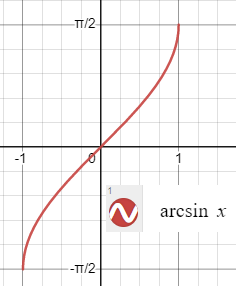
\includegraphics[width=0.4\textwidth]{trigonometrija.arcsin.png}
\centering
\end{figure}

\begin{figure}[H]
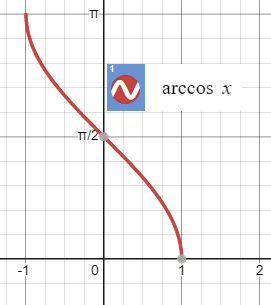
\includegraphics[width=0.4\textwidth]{trigonometrija.arccos.png}
\centering
\end{figure}

\begin{figure}[H]
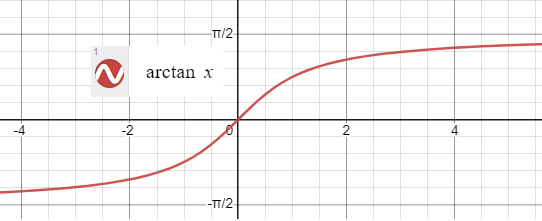
\includegraphics[width=0.6\textwidth]{trigonometrija.arctan.png}
\centering
\end{figure}

Veljajo zveze

\[\arcsin\sin x=x, x\in[-\frac{\pi}{2},\frac{\pi}{2}] \qquad \sin\arcsin x=x, x\in[-1,1]\]
\[\arccos\cos x=x, x\in[0,\pi] \qquad \cos\arccos x=x, x\in[-1,1]\]
\[\arctan\tan x=x, x\in(-\frac{\pi}{2},\frac{\pi}{2}) \qquad \tan\arctan x=x,x\in\mathbb{R}\]

\begin{zgled}
    Izračunajmo $\arcsin\frac{1}{2}=\frac{\pi}{6}$, $\arcsin(-1)=-\frac{\pi}{2}$, $\arcsin 4$ in preverimo s kalkulatorjem.
\end{zgled}
\begin{zgled}
    Izračunajmo $\arcsin(\sin\frac{7\pi}{6})=-\frac{\pi}{6}$.%ni na df ampak izberemo-pi/6
\end{zgled}
\begin{zgled}
    Izračunajmo $\arccos\frac{\sqrt{3}}{2}=\frac{\pi}{6}$.
\end{zgled}

\begin{zgled}
    Narišimo graf in povejmo lastnosti $f(x)=\arctan(x-1)-\frac{\pi}{2}$.
\end{zgled}
\begin{zgled}
    Izračunajmo $\arccos(\cos\frac{7\pi}{5})=\frac{3\pi}{5} (\neq \frac{7\pi}{5} \ \text{ker vrednost} \arccos\in[0,\pi]), \arcsin(\sin\frac{3\pi}{5})=\frac{2\pi}{5}$. (kalkulator)
\end{zgled}

\begin{example}
    464abc, 465abc, 466ad, 468abc, 469ab, 470abc, 473abc
\end{example}

Lastnosti vseh grafov krožnih funkcij (naraščanje, konkavnost, omejenost, Df, (asimptota)) doma.


\section{Trigonometrične enačbe}

\[\sin x=a \Rightarrow x_{k}^{1}=\arcsin a+2k\pi \land x_k^2=\pi-\arcsin a+2k\pi; k\in\mathbb{Z}\]

\begin{zgled}
    Rešimo enačbo $\sin x=\frac{\sqrt{3}}{2}$.
\end{zgled}

\begin{zgled}
    Poiščimo ničle $f(x)=2\sin(3x-\frac{\pi}{4})+1$ in $f(x)=2\sin(x)-\sqrt{2}$.
\end{zgled}

\[\cos x=a \Rightarrow x_k^1=\arccos a+2k\pi \land x_k^2=-\arccos a+2k\pi\]

\begin{zgled}
    Rešimo enačbo $\cos x=-\frac{\sqrt{3}}{2}$.
\end{zgled}

\begin{zgled}
    Rešimo enačbo $\cos\frac{x}{2} =\frac{1}{4}$.
\end{zgled}

\[\tan x=a\Rightarrow x_k=\arctan a+k\pi\]

Če imamo v enačbi različne kotne funkcije, poskusimo vse izraziti z eno (s pomočjo zvez npr. $\tan x=\frac{\sin x}{\cos x}, \sin^2x+\cos^2x=1,\ldots$, adicijskih izrekov, $\ldots$).

\begin{zgled}
    Rešimo enačbo $\tan x=\tan 10,\  \tan(\frac{1}{x})=1,\ \tan x=2\sin x$.
\end{zgled}

\begin{zgled}
    Rešimo enačbo $4\sin^2x+2\cos^2x=6-7\sin x$.
\end{zgled}

\begin{zgled}
    S faktoriziranjem razlike sinusov reši enačbo $\sin5x-\sin3x+\cos4x=0$.
\end{zgled}

\begin{zgled}
    Reši enačbo $\sin^2x+2\sin x\cos x-3\cos^2x=0$ (delimo s $\cos^2$)
\end{zgled}

\begin{zgled}
    Reši enačbo $\sin x=2\sin(x-\frac{\pi}{3})$, $\sin x \cos x=1$ in $\sin(2x)-\sin x=0$.
\end{zgled}

\begin{example}
    477be, 478a, 479abc, 481abcg, 484ab
\end{example}

\section{Naklonski kot med premicama}

Smerni koeficient premice $y=kx+n$, je enak $k=\tan\alpha$, kjer je $\alpha$ naklonski kot.\\

Naklonski kot $\phi$ med premicama (absolutna vrednost, ker iščemo ostri kot): 
\[\tan\phi=\tan(\alpha_1-\alpha_2)=\frac{\tan\alpha_2-\tan\alpha_1}{1+\tan\alpha_1\tan\alpha_2}=\frac{k_2-k_1}{1+k_1k_2},\]
\[\phi=\arctan|\frac{k_2-k_1}{1+k_1k_2}|\]

Spomnimo se $p||q\iff k_1=k_2$\qquad,\qquad  $p\perp q\iff k_1=-\frac{1}{k_2}$.

\begin{zgled}
    Izračunajmo naklonski kot med premicama $y=\frac{1}{3}x+1$ in $y=2x-3$.
\end{zgled}

\begin{example}
    \fbox{491a}bcč, \fbox{492ab}c, \fbox{493}, 494, \fbox{496}
\end{example}


\end{document}